\documentclass[12pt]{article}
\usepackage{mc}
\mcheader{Grades 4--5}

% writing space: \space{height in cm}
\newcommand{\workbox}[1]{%
  \begin{tikzpicture}\draw[box] (0,0) rectangle (17.6,-#1);\end{tikzpicture}%
}

% pair grid: \pairgrid{max}{cell}
\newcommand{\pairgrid}[2]{%
  \begin{tikzpicture}[baseline=(current bounding box.north)]
    \foreach \i in {0,...,#1}{%
      \fill[black!8] ({(\i+1)*#2},0) rectangle ++(#2,-#2);
      \draw[cell] ({(\i+1)*#2},0) rectangle ++(#2,-#2);
      \node at ({(\i+1.5)*#2},{-0.5*#2}) {\i};
      \fill[black!8] (0,{-(\i+1)*#2}) rectangle ++(#2,-#2);
      \draw[cell] (0,{-(\i+1)*#2}) rectangle ++(#2,-#2);
      \node at ({0.5*#2},{-(\i+1.5)*#2}) {\i};
      \foreach \j in {0,...,#1}{%
        \draw[cell] ({(\j+1)*#2},{-(\i+1)*#2}) rectangle ++(#2,-#2);
      }
    }
    \node[anchor=south] at ({(#1+3)*#2/2},0.05) {other pile};
    \node[anchor=south, rotate=90] at (-0.05,{-(#1+3)*#2/2}) {one pile};
  \end{tikzpicture}%
}

\begin{document}
\fontsize{12}{16.5}\selectfont

Each game is for two players and a pile of counters. The players take turns taking counters from the pile. Whoever takes the last counter wins.

\vspace{10pt}
\problem Each turn takes 1 or 2 counters. For every starting pile from 1 to 15 counters, decide whether you would rather go first or second, and write 1st or 2nd under the number. Then decide what you would choose with 100 counters, and explain why your way of playing wins whatever your partner does.

\vspace{4pt}
\numtable{1}{15}{15}{1.17}{0.7}{1.0}{0.4}

\vspace{6pt}
\workbox{4.1}

\vspace{14pt}
\problem A pile is called a winning pile if the player about to move can be sure to win from it, and a losing pile if not. Now each turn takes 1, 3, or 4 counters. Write W or L under each pile from 1 to 30. Describe the pattern, and explain why it continues forever.

\vspace{4pt}
\numtable{1}{30}{15}{1.17}{0.7}{1.0}{0.35}

\vspace{6pt}
\workbox{3.9}

\newpage
\problem Here are seven rules. For each rule, circle the losing piles from 1 to 24. Some of the rules have exactly the same losing piles. Find them, and for one such pair of rules explain why their losing piles are the same.

\vspace{8pt}
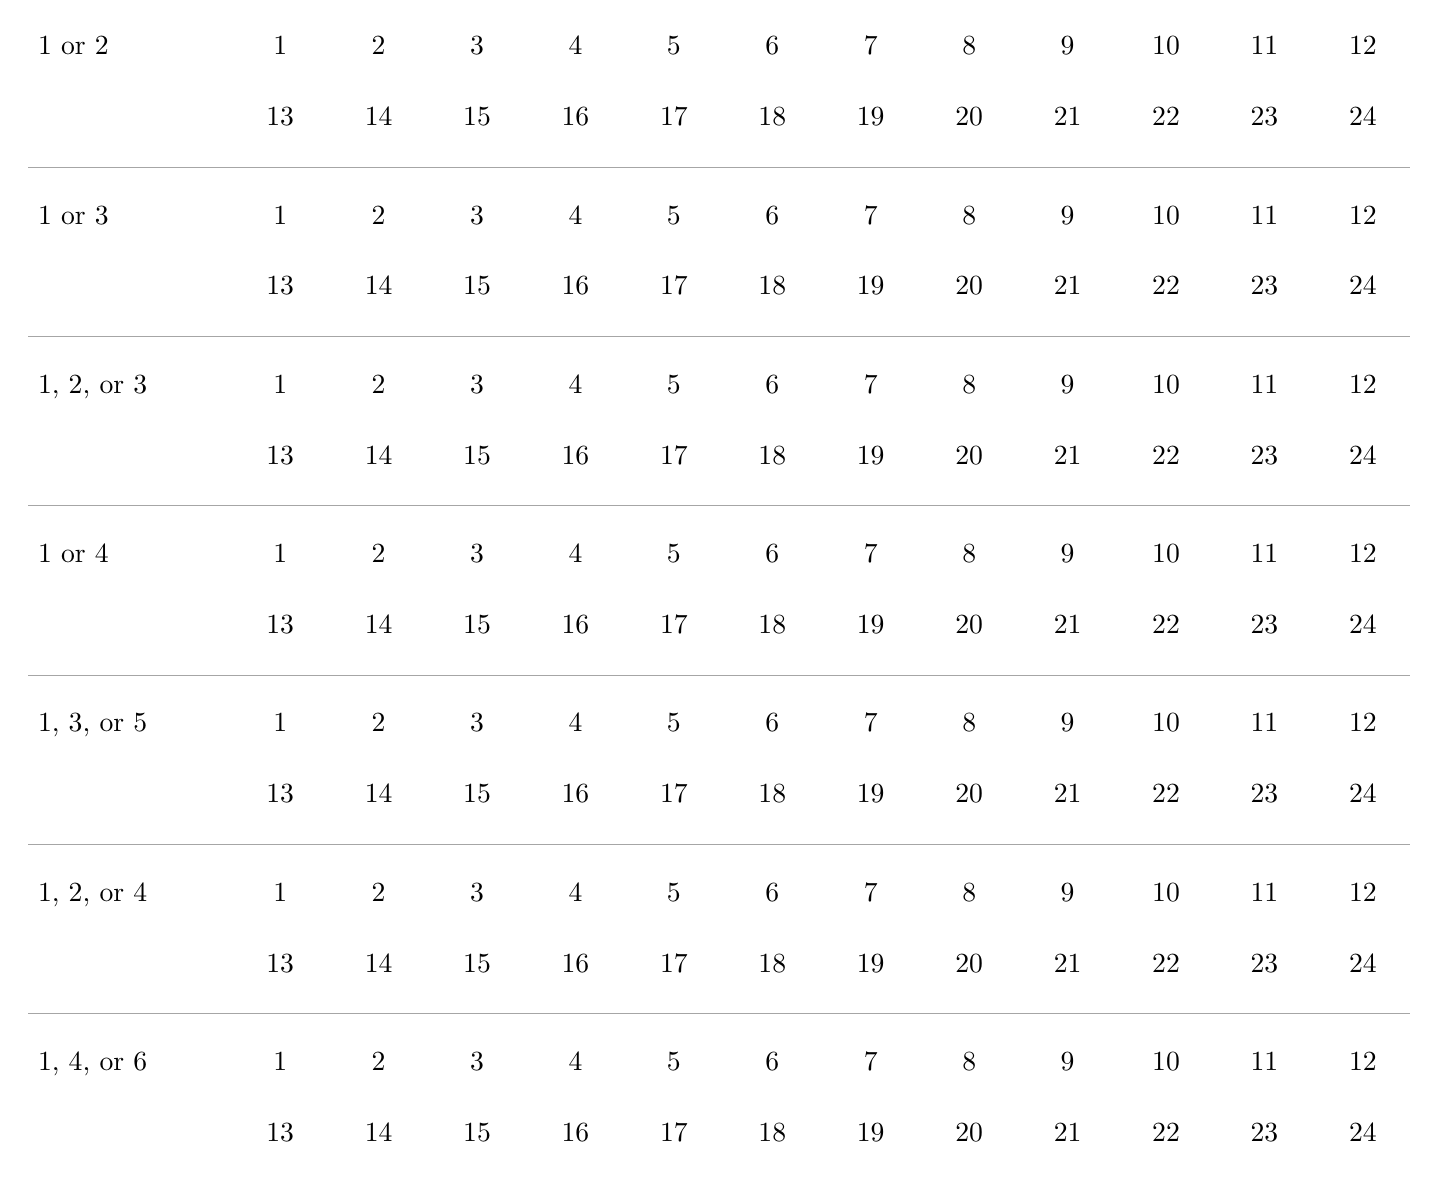
\begin{tikzpicture}
  \foreach \t [count=\r from 0] in {{1 or 2},{1 or 3},{1, 2, or 3},{1 or 4},{1, 3, or 5},{1, 2, or 4},{1, 4, or 6}}{%
    \pgfmathsetmacro{\yy}{-\r*2.15}%
    \node[anchor=base west] at (0,\yy) {\t};
    \foreach \k in {1,...,12}{%
      \node[anchor=base] at ({3.2+(\k-1)*1.25},\yy) {\k};
    }
    \foreach \k in {13,...,24}{%
      \node[anchor=base] at ({3.2+(\k-13)*1.25},\yy-0.9) {\k};
    }
  }
  \foreach \r in {1,...,6}{%
    \draw[line width=0.4pt, black!35] (0,{-\r*2.15+0.72}) -- (17.55,{-\r*2.15+0.72});
  }
\end{tikzpicture}

\vspace{10pt}
\workbox{5.2}

\newpage
\problem Kai always takes as many counters as the rule allows. With the rule 1, 3, or 4, list every winning pile from 1 to 30 where Kai's move is a mistake. For which of the seven rules in Problem 3 is Kai's move from a winning pile never a mistake? Explain why for one of them.

\vspace{6pt}
\workbox{5.6}

\vspace{14pt}
\problem For each list of losing piles below, find a rule that includes taking 1 and has exactly these losing piles, with the list continuing in the same way forever. If no rule works, explain why.

\vspace{6pt}
\begin{tikzpicture}
  \foreach \t [count=\j from 0] in {{5, 10, 15, 20, 25, 30, \dots},{2, 8, 10, 16, 18, 24, \dots},{3, 7, 10, 14, 17, 21, \dots},{3, 5, 8, 10, 13, 15, \dots}}{%
    \pgfmathtruncatemacro{\col}{mod(\j,2)}%
    \pgfmathtruncatemacro{\row}{floor(\j/2)}%
    \pgfmathsetmacro{\bx}{\col*8.95}%
    \pgfmathsetmacro{\by}{-\row*6.1}%
    \draw[box] (\bx,\by) rectangle ++(8.65,-5.8);
    \node[anchor=north west, font=\large] at (\bx+0.3,\by-0.3) {\t};
  }
\end{tikzpicture}

\newpage
\problem Each turn takes 1, 6, or 9 counters. Write W or L under each pile from 1 to 40, and find where the pattern starts to repeat. Then explain why, for every rule, the pattern of W and L must repeat from some point on.

\vspace{4pt}
\numtable{1}{40}{20}{0.88}{0.65}{0.95}{0.35}

\vspace{6pt}
\workbox{4.6}

\vspace{14pt}
\problem Now there are two piles. Each turn takes 1 or 2 counters from one of the piles, and whoever takes the very last counter wins. In the grid, write W or L for each pair of piles with 0 to 7 counters each. Describe all the losing pairs, and explain why they are losing.

\vspace{10pt}
\hspace*{0.6cm}\pairgrid{7}{0.82}\hfill
\begin{tikzpicture}[baseline=(current bounding box.north)]\draw[box] (0,0.45) rectangle (7.6,-6.6);\end{tikzpicture}

\newpage
\problem Two piles again, but now each turn takes 1, 3, or 4 counters from one of the piles. Write W or L for each pair of piles with 0 to 8 counters each. Then list every losing pair where the two piles have different sizes.

\vspace{10pt}
\hspace*{0.6cm}\pairgrid{8}{0.95}\hfill
\begin{tikzpicture}[baseline=(current bounding box.north)]\draw[box] (0,0.45) rectangle (6.4,-9.05);\end{tikzpicture}

\newpage
\problem Each turn still takes 1, 3, or 4 counters. Label each single pile as follows. An empty pile is labeled 0. Any other pile is labeled with the smallest of 0, 1, 2, 3, \dots\ that is not the label of a pile you can move to. Find the labels of the piles from 0 to 20, and find how they tell you which pairs in your grid from Problem 8 are losing pairs. Then decide whether piles of 11 and 13 counters make a winning pair or a losing pair, do the same for piles of 12 and 18 counters, and explain your answers.

\vspace{4pt}
\numtable{0}{20}{11}{1.6}{0.7}{1.0}{0.35}

\vspace{6pt}
\workbox{11.0}

\end{document}
